
\setcounter{chapter}{8}

\chapter{Constructing and sharing grounded categories}
\label{c:grounded-categories}
\label{c:ggg}

In the previous Chapter we investigated what it takes to do apply the
non-grounded Naming Game from Chapter \ref{c:naming-game} (page
\pageref{c:naming-game}) to a robotic setup and it turned out that --
although word representations and alignment mechanisms remained
unchanged -- quite complex cognitive representations and mechanisms
were needed for acquiring grounded notions of individual objects. In
this chapter we will investigate how the multi-word utterances and
structured word representations from Chapter \ref{c:gg} (page
\pageref{c:gg}) can be connected to categories that are grounded in
the world of our robots and how these categories can be aligned
through language.

This will introduce three major challenges in constructing and
maintaining of semiotic networks. First, agents need to be able to
construct ontologies of meaningful \emph{perceptual categories} such
as \texttt{red} and \texttt{small} from their sensory
experiences. Second, they need conceptualization mechanisms that find
combinations of these categories that discriminate the topic from the
other objects in the context. And third, word alignment dynamics need
to take into account that each agent individually constructs such
categories from noisy perceptions and thus the success of words in the
population also depends on how conventionalized the underlying
categories are.


\section{Categorization strategies}

We discussed in detail what it means to ``construct grounded
categories'' in Section \ref{s:saussure-to-peirce} on page
\pageref{s:saussure-to-peirce} and also listed a few common techniques
to implement categorization mechanism in robots in the subsequent
Section \ref{s:mental-representations-for-categorizations}. Since the
focus of our work is on lexicon formation, we will only briefly cover
this topic. In order to show that the lexicon formation strategies are
independent from the categorization strategies, we will introduce and
compare two grounded category representations, namely
\emph{discrimination trees} and \emph{prototypes}, which both assign
intervals on sensory channels to categories and thus allow for
distinctions such as \texttt{small} vs \texttt{big}, \texttt{green}
vs. \texttt{red}, and so on.

~\\

\noindent For all experiments in this chapter, we use the same robotic
setup and the same overall language game script as in the previous
chapter. As in all of the previous chapters, we will only describe the
differences in strategies.

\inparagraph{Discrimination trees} This categorization technique was
introduced by
\citealp{steels98origins-ontologies,steels97grounding,steels99situated,steels97constructing}
for the Talking Heads experiment. Categories are formed by recursively
splitting a sensory channel into intervals of same length (see Figure
\ref{f:category-representations}a), that is, an ontology $O(a)$ of an
agent $a$ consists of a set of categories $c(a)$ that assign an
interval $]min, max], 0 \leq min < max \leq 1$ to a sensory channel
with a score $\delta$ that reflects how successful the category was
used in previous communicative interactions. In the example in Figure
\ref{f:category-representations}a, the category \texttt{c-9} covers
the interval between 0 and 0.25 on the \texttt{green-red} channel and
thus can be used to refer to ``very green'' objects. A category is
\emph{applicable} to an object when the sensory value for the channel
of the category falls within the interval of the category.

\begin{figure}[t]
  \centerline{\begin{tabular}{ll}
    a) & b) \\
    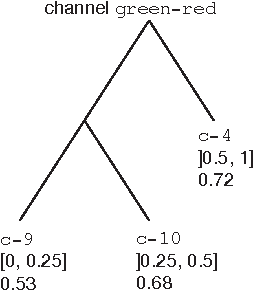
\includegraphics[height=0.3\textwidth]{figures/discrimination-tree}\hspace{2cm} &
    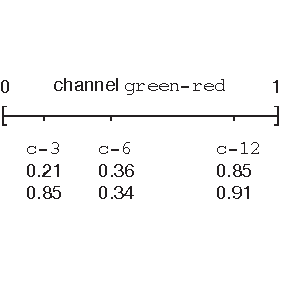
\includegraphics[height=0.3\textwidth]{figures/prototype}
  \end{tabular}}
    \caption{Assigning areas on sensory channels to categories using a) discrimination trees and b) prototypes}
  \label{f:category-representations}
\end{figure}




\inparagraph{Prototypes} As an alternative category representation we
also implemented something that resembles the continuous category
membership of the basic level categories of \cite{rosch73natural} and
which was applied in similar form to Lego robots by
\cite{vogt03anchoring}. In this strategy, a category $c(a)$ is
characterized by a single point $0 \leq v \leq 1$ on a sensory channel
and again a score $\delta$ that reflects communicative success. The
points on the sensory channel spans a one-dimensional Voronoi region,
i.e. a category is applicable to an object if it is closest to the
perceived sensory value of the object among all prototypes on the same
channel. In the example of Figure \ref{f:category-representations}b,
the prototypical value of the category \texttt{c-6} is 0.36, with a
score of 0.34. Considering the values of the other categories on the
\texttt{green-red} channel, this means that all objects that have a
sensory value between 0.29 (the middle between \texttt{c-3} and
\texttt{c-6}) and 0.61 (between \texttt{c-6} and \texttt{c-12}) will
be categorized as \texttt{c-6}.


\inparagraph{Conceptualization} Speakers who attempt to construct a
meaning representation that discriminates the topic from the other
objects in the sensory context follow the same strategy as in the
non-grounded version of the experiment in Chapter \ref{c:gg} (see
Section \ref{s:sgg-sw-unstructured-conceptualization} on page
\pageref{s:sgg-sw-unstructured-conceptualization}). That is, they try
to find combinations of categories that are applicable to the topic
but not to the other objects. The only difference is that in the
non-grounded version the categories are already part of the perceived
simulated objects, whereas in the grounded version each agent
individually needs to determine which of his categories are applicable
and which not.


\inparagraph{Saliency \& conventionalization} When dealing with
real-world perceptions, some combinations of categories are better
conceptualizations of a scene than others. This is for three reasons:
first, the perceived difference between the topic and the other
objects in the context can be very different for different channels
and thus categories on these perceptual channels lead to a more
contrasting descriptions of an object. This can be captured by
computing a \emph{saliency} measure as the minimum distance on the
channel of a category between the topic and the other objects in the
context. Second, some categories are better conventionalized in the
population and thus it is beneficial to prefer them over other
categories. This is captured by the aforementioned category score
score that is updated as an outcome of the game (see below). And
third, in the case of prototypes, the distance between perceived
channel values and the prototype can be used as a measure of how well
a category expresses a topic. These criteria are combined into a
meaning score by multiplying the measures and averaging the result
over all categories of a meaning.


\inparagraph{Extending the ontology} All agents start without any
categories and obviously mechanisms are needed to extend
ontologies. For this, \cite{steels99situated} used a failure in
conceptualizing a scene as a trigger to invent new categories. The
problem with this strategy is that agents might continue to use less
suited categories that nevertheless allow conceptualization and thus
get stuck with suboptimal solutions.  A better strategy is to create
new categories whenever they would increase the overall meaning
score. For this, agents conceptualize a scene with their existing
categories but also also try to conceptualize with new categories that
were created for the most salient channels. Only when a new category
leads to a meaning with a higher combined meaning score, then it is
added to the ontology.

\inparagraph{Production, parsing and word learning} All other
mechanisms for processing and maintaining semiotic networks in
production, interpretation and alignment remain unchanged from Chapter
\ref{c:gg}. We will immediately assume the case of multi-word
utterances for structured word meanings.


\inparagraph{Ontology alignment} After each interaction, the speaker
and hearer update the scores of the categories involved in their
respective meaning representations to reflect how well they are
conventionalized in the population. For that, the scores of the
categories that were part of the meaning that was expressed by the
speaker and interpreted by the hearer are increased by a fixed value
of $0.02$ in case of success and decreased by $0.02$ in case of
failure. Categories with a score of $0$ are removed from the
ontology. Furthermore, when prototypes are used for categorization,
their values are slightly shifted towards the perceived value of the
topic in order to better reflect the distribution of feature values in
the environment (analogously to the shifting of prototypes described
in Section \ref{s:gng-prototypes} on page \pageref{s:gng-prototypes}).


\section{Problems in aligning fixed form-meaning mappings}

To demonstrate that the categorization mechanisms and the interplay of
categories and words indeed work, we first ran the model with a
modification in which both the speaker and hearer artificially have
the same perception of a scene and thus perceptual differences do not
play a role. That is, before each interaction, both agents are fed
with the perception of the same randomly chosen robot from a recorded
scene.

\begin{figure}[t]
  \gnuplotfigure{figures/ggg-dt-mw-structured-same-perception-success+lexicon+ontology}
  \caption{Main alignment dynamics with discrimination trees and
    shared perceptions. Communicative success (measure
    \ref{m:communicative-success}), lexicon size
    (\ref{m:lexicon-size}), ontology size (\ref{m:ontology-size}) and
    discrimination tree lexicon coherence (measure
    \ref{m:lexicon-coherence-discrimination-trees}) are averaged
    across 10 repeated series of 25000 interactions.}
  \label{f:ggg-dt-mw-structured-same-perception-success+lexicon+ontology}
\end{figure}


\begin{measure}[b]{Ontology size}{m:ontology-size}
  Measures the number of categories in the ontology of agents averaged
  over all agents of the population: $$v = \frac{\sum_{i=1}^{|P|}
    |O(a_i)|}{|P|}$$ Values $v$ are averaged over the last 250
  interactions.
\end{measure}

\begin{figure}[t]
  \gnuplotfigure{figures/ggg-p-mw-structured-same-perception-success+lexicon+ontology}
  \caption{Main alignment dynamics with prototypes and shared
    perceptions. Communicative success (measure
    \ref{m:communicative-success}), lexicon size
    (\ref{m:lexicon-size}), ontology size (\ref{m:ontology-size}) and
    lexicon coherence for prototypes (measure
    \ref{m:lexicon-coherence-prototypes}) are averaged
    across 10 repeated series of 25000 interactions.}
  \label{f:ggg-p-mw-structured-same-perception-success+lexicon+ontology}
\end{figure}


\begin{measure}[b]{Lexicon coherence for discrimination
    trees}{m:lexicon-coherence-discrimination-trees}
  Provides a measure for how similar the meanings underlying the
  lexicons of the interacting agents are. This measure is identical to
  measure \ref{m:lexicon-coherence} on page
  \pageref{m:lexicon-coherence}, with the assumption that two
  categories in the ontologies of two different agents are ``equal''
  when they cover the same interval on the same sensory channel.
\end{measure}

\begin{measure}[b]{Lexicon coherence for
    prototypes}{m:lexicon-coherence-prototypes}
  Measures the prototype similarity between the word meanings of the
  speaker and hearer of an interaction. The average distance between
  the prototype values of the meanings of the words that overlap in
  form between speaker and hearer is divided by the average number of
  words in the two agents' lexicons.
\end{measure}


The overall alignment dynamics for agents that use discrimination
trees are shown in Figure
\ref{f:ggg-dt-mw-structured-same-perception-success+lexicon+ontology}. In
the first few thousand interactions, the agents quickly acquire a set
of around 25 categories, a number that later only slightly increases
because we limited the depth of discrimination trees to two (higher
depths also work well). Compared to the non-grounded version of this
experiment (see Figure \ref{f:sgg-mw-structured-success+lexicon-size}
on page \pageref{f:sgg-mw-structured-success+lexicon-size}),
communicative success and coherence are reached as quickly or even
quicker and the maximum number of words that the agents invent or
adopt is only 50\% higher than the number of categories (compared to
around 800\% in the non-grounded version). 

On the first sight this is surprising, since there is the additional
challenge of creating grounded categories. However, because speaker
and hearer always have the same perception of a scene and because they
use the same way to split the sensory channels into categories, all
agents in the population end up adopting the same
categories. Furthermore, because the incorporation of saliency in the
criteria for selecting meanings from alternative conceptualizations,
speaker and hearer almost always conceptualize a scene in the same way
(only due to different category scores different conceptualizations
can occur, which accounts for the fact that a very small fractions
still fail after 10000 interactions). Consequently, the problem of
referential uncertainty almost does not exist when agents have shared
perceptions because the distributional structure of sensory values
across the objects largely narrows down the hypothesis space.



When prototypes are used for categorization, the results are very
similar (see Figure
\ref{f:ggg-p-mw-structured-same-perception-success+lexicon+ontology}). The
number of categories created and thus lexicon size are slightly
lower. Because now each agent individually partitions sensory channels
in varying number of categories and thus more different
conceptualizations of a scene are possible, coherence and
communicative success are slightly lower than when using
discrimination trees.


~\\

\begin{figure}[t]
  \gnuplotfigure{figures/ggg-dt-mw-structured-category-channel-entrenchment}
  \caption{Success of categories in communication per sensory channel.
    For all categories of the first agent in the population, the
    average scores of all categories are plotted per channel along the
    x axis.}
  \label{f:ggg-dt-mw-structured-category-channel-entrenchment}
\end{figure}

\begin{figure}[p]
  \rotatebox{90}{
\renewcommand{\arraystretch}{1.3}{
\hskip0.2cm\begin{tabular}{lllp{3.7cm}llp{3.7cm}lc}
  \\[1.0em]
  \# & speaker & topic & meaning & utterance & hearer & meaning & topic & success? \\
  \hline
5000 & agent 6 & \texttt{obj-69} & \texttt{[y-1: 0.26]} & \textit{``nakexo''} & agent 10 &  & \texttt{} & no \\
5001 & agent 4 & \texttt{obj-7} & \texttt{[yellow-blue-2: 1.00]}

\texttt{[green-red-2: 1.00]} & \textit{``renefi romive''} & agent 2 & \texttt{[yellow-blue-2: 1.00]}

\texttt{[green-red-2: 1.00]} & \texttt{obj-7} & yes \\
5002 & agent 7 & \texttt{obj-31} & \texttt{[width-1: 0.18]} & \textit{``zanuta''} & agent 6 &  & \texttt{} & no \\
5003 & agent 3 & \texttt{obj-18} & \texttt{[y-2: 0.04]} & \textit{``luxoza''} & agent 7 & \texttt{[luminance-1-2: 0.28]} & \texttt{} & no \\
5004 & agent 10 & \texttt{obj-160} & \texttt{[height-1: 0.64]} & \textit{``mazilu''} & agent 3 & \texttt{[height-1: 0.76]} & \texttt{} & no \\
5005 & agent 9 & \texttt{obj-134} & \texttt{[height-2: 0.94]} & \textit{``wofoza''} & agent 10 & \texttt{[height-2: 0.48]} & \texttt{} & no \\
5006 & agent 1 & \texttt{obj-3} & \texttt{[luminance-2: 0.28]} & \textit{``tetupi''} & agent 2 & \texttt{[yellow-blue-2: 0.98]}

\texttt{[height-1: 0.62]} & \texttt{} & no \\
5007 & agent 7 & \texttt{obj-131} & \texttt{[yellow-blue-2: 1.00]}

\texttt{[green-red-2: 1.00]} & \textit{``romive renefi''} & agent 4 & \texttt{[green-red-2: 1.00]}

\texttt{[yellow-blue-2: 1.00]} & \texttt{obj-133} & yes \\
5008 & agent 5 & \texttt{obj-174} & \texttt{[green-red-1: 1.00]} & \textit{``xubifu''} & agent 7 & \texttt{[green-red-1: 0.98]} & \texttt{obj-178} & yes \\
5009 & agent 10 & \texttt{obj-57} & \texttt{[green-red-1: 1.00]} & \textit{``xubifu''} & agent 5 & \texttt{[green-red-1: 1.00]} & \texttt{obj-47} & yes \\
5010 & agent 5 & \texttt{obj-49} & \texttt{[green-red-2: 0.98]} & \textit{``renefi''} & agent 9 & \texttt{[green-red-2: 0.98]} & \texttt{} & no \\
5011 & agent 1 & \texttt{obj-110} & \texttt{[green-red-1-1: 0.38]} & \textit{``gawude''} & agent 4 & \texttt{[green-red-1-1: 0.36]} & \texttt{obj-111} & yes \\
5012 & agent 9 & \texttt{obj-7} & \texttt{[width-2: 0.26]} & \textit{``renefi''} & agent 3 & \texttt{[green-red-2: 1.00]} & \texttt{obj-9} & yes \\
5013 & agent 8 & \texttt{obj-163} & \texttt{[green-red-2: 1.00]} & \textit{``renefi''} & agent 10 & \texttt{[green-red-2: 1.00]} & \texttt{obj-159} & yes \\
5014 & agent 2 & \texttt{obj-120} & \texttt{[yellow-blue-1: 1.00]} & \textit{``radila''} & agent 5 & \texttt{[yellow-blue-1: 1.00]} & \texttt{obj-120} & yes \\
5015 & agent 9 & \texttt{obj-35} & \texttt{[height-1-1: 0.44]} & \textit{``busimu''} & agent 10 & \texttt{[y-2: 0.06]} & \texttt{obj-44} & yes \\
5016 & agent 9 & \texttt{obj-172} & \texttt{[green-red-2: 1.00]} & \textit{``renefi''} & agent 1 & \texttt{[green-red-2: 1.00]} & \texttt{obj-176} & yes \\
5017 & agent 2 & \texttt{obj-215} & \texttt{[yellow-blue-1: 1.00]} & \textit{``radila''} & agent 5 & \texttt{[yellow-blue-1: 1.00]} & \texttt{obj-218} & yes \\
5018 & agent 10 & \texttt{obj-163} & \texttt{[green-red-2: 0.98]}

\texttt{[luminance-1-2: 0.36]} & \textit{``pogupu renefi''} & agent 1 & \texttt{[green-red-2: 0.98]} & \texttt{} & no \\
5019 & agent 1 & \texttt{obj-87} & \texttt{[green-red-2: 1.00]} & \textit{``renefi''} & agent 4 & \texttt{[green-red-2: 1.00]} & \texttt{obj-87} & yes \\
\\[1.0em]
 \\\end{tabular}}


%%% Local Variables: 
%%% mode: latex
%%% TeX-master: "../phd-thesis"
%%% End: 


}
  \caption{Overview of 20 consecutive interactions in a population of
    10 agents from game 5000 on. It shows the agents that are
    interacting, the topic chosen by the speaker, the conceptualized
    meaning that was chosen, the utterance, the meaning parsed by the
    hearer together with the interpreted topic, and whether the agents
    reached communicative success.}
  \label{f:ggg-mw-structured-trace}
\end{figure}

\noindent However, when removing the scaffold of providing the agents
with the same perception of a scene, agents that use the strategies
described in the previous section are much less successful in agreeing
on communication systems. Responsible for this is the high perceptual
deviation, i.e. the differences in the visual perceptions of physical
objects by the two interacting robots. This difference is
systematically higher for some sensory channels that for others (see
Figure \ref{f:data-sets-perceptual-deviation-matrix} on page
\pageref{f:data-sets-perceptual-deviation-matrix}). The correlation
between the perception of robots is highest for the
\texttt{yellow-blue} and \texttt{green-red} sensory channels, and it
is lowest for the \texttt{x} and \texttt{y} channels. By incorporating
feedback from the use in language, agents learn to rely more on highly
correlating channels, as shown in Figure
\ref{f:ggg-dt-mw-structured-category-channel-entrenchment}. The
average category scores are highest for categories on the
\texttt{yellow-blue} and \texttt{green-red} channels and lowest for
categories on the \texttt{width}, \texttt{x} and \texttt{y} channels,
which directly mirrors the distributions in sensory deviation.


\begin{figure}[t]
  \gnuplotfigure{figures/ggg-dt-mw-structured-problems}
  \caption{Sources of alignment problems. The frequency of word
    adoptions by the hearer (measure \ref{m:word-adoptions-hearer}),
    the number of interactions in which agents succeeded but used
    different meanings (measure
    \ref{m:succeeded-with-different-meanings}) and the number of times
    interactions failed with the same meaning (measure
    \ref{m:failed-with-same-meanings}) are averaged over 10 repeated
    series of 25000 interactions}
  \label{f:ggg-dt-mw-structured-problems}
\end{figure}


\begin{measure}[b]{Number of word adaptions
    hearer}{m:word-adoptions-hearer}
  Another measure for lexicon stability. Whenever the hearer adopts a
  new word meaning as the result of a failed communicative
  interaction, the value of 1 is recorded, otherwise 0. Values are
  averaged over the last 250 interactions.
\end{measure}

\begin{measure}[b]{Communicative failure with same
    meanings}{m:failed-with-same-meanings}
  Measures the fraction of interactions in which agents did not reach
  communicative success although the hearer parsed the utterance into
  a the same meaning as the one that was conceptualized by the
  speaker. After each interaction, the value of 1 is recorded when
  communicative success was not reached (see measure
  \ref{m:communicative-success}) and when the meaning that underlies
  the utterance produced by the speaker is identical (categories on
  the same sensory channel cover the same categories) to the meaning
  that was used by the hearer to interpret the topic. Otherwise, a
  value of 0 is recorded. Values are averaged over the last 250
  interactions.
\end{measure}


Nevertheless, although the alignment mechanisms are sensitive to
different degrees of sensory deviation, the lateral inhibition based
word meaning selection process is constantly faced with the problem of
inconsistent categorization and ``wrong'' feedback, which adds great
difficulties to the problems already inherent in the lexicon formation
model. This is illustrated in Figure \ref{f:ggg-mw-structured-trace},
which shows traces of 20 interactions from game 5000 on. For example
in interaction 5005, both agents assume the meaning of ``wofoza'' to
be a category that covers the interval between 0.5 and 1 on the
\texttt{height} channel, but nevertheless the interaction fails,
because the category was not applicable to the hearer's perception of
the scene. Analogously, interaction 5012 is an example of the
opposite. Although the categories that are associated by speaker and
hearer to the form ``renefi'' are on different sensory channels, the
communication still resulted in a communicative success. In both
cases, the wrong entities in the semiotic networks of both agents are
increased or respectively decreased in score, which makes it very hard
to reach coherence.


\begin{figure}[t]
  
{\renewcommand{\arraystretch}{1.5}
\begin{tabular}{@{}p{1cm}|p{3cm}@{}p{0.6cm}@{}|p{3.0cm}@{}p{0.6cm}@{}|p{3.0cm}@{}p{0.6cm}@{}}
form & agent 1 &  & agent 2 &  & agent 3 & \\
\hline
\textit{``poxiga''}&\texttt{[yellow-blue-2: 1.00] [green-red-2: 1.00]}
&0.50&\texttt{[yellow-blue-1: 1.00] [green-red-2: 1.00]}


\texttt{[y-1: 0.22]}
&0.50

0.30&\texttt{[y-1: 0.22]}
&0.30\\
\hline
\textit{``watave''}&\texttt{[x-1: 0.22]}
&0.40&&&&\\
\hline
\textit{``genuke''}&\texttt{[height-1: 0.78]}
&0.30&\texttt{[luminance-1-1: 0.26]}
&0.30&&\\
\hline
\textit{``wavimu''}&\texttt{[luminance-1-2: 0.28]}
&0.50&&&\texttt{[height-1-2: 0.38]}
&0.40\\
\hline
\textit{``pifizi''}&\texttt{[yellow-blue-1: 1.00] [green-red-1: 1.00]}
&0.30&\texttt{[height-1-1: 0.36]}


\texttt{[luminance-1-2: 0.38]}
&0.30

0.30&\texttt{[luminance-2: 0.14]}


\texttt{[green-red-1-1: 0.32]}
&0.50

0.20\\
\hline
\textit{``tubafi''}&\texttt{[y-2: 0.12]}
&0.20&&&&\\
\hline
\textit{``gazomi''}&\texttt{[width-1: 0.16]}
&0.20&\texttt{[luminance-1: 0.32]}
&0.30&\texttt{[width-1: 0.16]}
&0.40\\
\hline
\textit{``gapemu''}&\texttt{[x-1: 0.22]}
&0.40&\texttt{[y-2: 0.10]}
&0.40&\texttt{[green-red-1: 1.00] [y-1: 0.22]}
&0.50\\
\hline
\textit{``runese''}&\texttt{[y-2: 0.12]}
&0.20&\texttt{[yellow-blue-2: 1.00] [width-1-2: 0.34]}
&0.40&\texttt{[yellow-blue-2: 1.00] [width-1-1: 0.28]}


\texttt{[green-red-1-1: 0.32]}
&0.30

0.40\\
\hline
\textit{``kuvuka''}&\texttt{[width-1-2: 0.28]}
&0.50&\texttt{[width-2: 0.26]}
&0.10&&
\end{tabular}}


%%% Local Variables: 
%%% mode: latex
%%% TeX-master: "../phdbook"
%%% End: 

  \caption{The associated categories and word association scores of
    the first 10 words of agent 1 (out of a population of 10 agents)
    and the corresponding meanings in the lexicons of agents 2 and 3
    after 5000 interactions. }
  \label{f:ggg-mw-structured-lexicon-forms-5000}
\end{figure}



More than 10 percent of the interactions fail despite the meanings
that were conceptualized or interpreted cover the same categories on
the same interval on the same channels, as shown in Figure
\ref{f:ggg-dt-mw-structured-problems}. And initially 10 percent and
later 5 percent of the interactions succeed although the meanings
covered different intervals or other channels. With this inconsistent
feedback, hearers still adopt new word meanings in 40 percent of the
interactions even after 10000 interactions.  As a consequence, the
agents are not able to construct stable and coherent lexicon
representations, as illustrated by the lexicon snapshots in Figure
\ref{f:ggg-mw-structured-lexicon-forms-5000}. Although after 5000
interactions on average each agent already took part in 1000
interactions, non of the first 10 word meanings of agent 1 are shared
by agent 2 and 3.



\startfiguregroup
  
\begin{figure}[t]
  \gnuplotfigure{figures/ggg-dt-mw-structured-success+lexicon+ontology}
  \caption{Main alignment dynamics for agents that use discrimination
    trees for categorization. Communicative success (measure
    \ref{m:communicative-success}), lexicon size
    (\ref{m:lexicon-size}), ontology size (\ref{m:ontology-size}) and
    discrimination tree lexicon coherence (measure
    \ref{m:lexicon-coherence-discrimination-trees}) are averaged
    across 10 repeated series of 25000 interactions.}
  \label{f:ggg-dt-mw-structured-success+lexicon+ontology}
\end{figure}


\begin{figure}[t]
  \gnuplotfigure{figures/ggg-p-mw-structured-success+lexicon+ontology}
  \caption{Main alignment dynamics with prototypes. Communicative
    success (measure \ref{m:communicative-success}), lexicon size
    (\ref{m:lexicon-size}), ontology size (\ref{m:ontology-size}) and
    lexicon coherence for prototypes (measure
    \ref{m:lexicon-coherence-prototypes}) are averaged across 10
    repeated series of 25000 interactions.}
  \label{f:ggg-p-mw-structured-success+lexicon+ontology}
\end{figure}

\stopfiguregroup


Not surprisingly, the overall alignment dynamics completely break down
when agents individually perceive real-world scenes (see Figure
\ref{f:ggg-dt-mw-structured-success+lexicon+ontology} and
\ref{f:ggg-p-mw-structured-success+lexicon+ontology}).  Lexicon
coherence hovers between 10 and 15 percent, and due to the permanent
adoption of new word meanings, later inhibition dynamics are not able
to stop a continuous increase in lexicon size. The communicative
success for agents that use prototypes (70\%) is slightly higher than
when discrimination trees are used (60\%), which is because
discrimination trees cut sensory channels at fixed points, whereas
prototypes allow to cut sensory channels into intervals that are more
robust against perceptual deviation. For example discrimination tree
category can never cover an interval between 0.35 and 0.6, wheres a
prototype can. When for a specific channel many values occur around
the value of 0.5, then the prototype is better applicable to these
objects.

Given such low levels of coherence and communicative success, we omit
the analysis of scaling behavior for this model.


%%% Local Variables: 
%%% mode: latex
%%% TeX-master: "phd-thesis"
%%% End: 
